% Appendix A27 --- cross-source generalisation and skin-tone fairness (supplementary analysis).
% Source-of-truth (ICLR re-run only, R10-compliant; BMVC cross-domain/fairness numbers NOT reused):
%   - Skin-tone fairness: project/results/fairness_fitzpatrick_iclr_full.csv (ICLR-exclusive).
%   - Cross-source AUC:   project/results/external_*_predictions.csv (Jun14-15 ICLR re-run;
%                         per-source AUC independently recomputed via Bash, audited).
% Framing: honest boundary analysis, NOT a performance win. Absolute AUC is low because
%   Fitzpatrick17k / the pooled cross-source set is a hard, diverse clinical pool; the point is the
%   RELATIVE disparity across skin tones and the UNEVEN reach across acquisition sources, not high scores.
% Scope: fairness reports AUC differences ONLY (no ECE / calibration -- deferred, unresolved tension).
% This appendix is supplementary; it does not alter the main claims C1 (diagnosis preservation) and
%   C2 (query-for-retake closed loop).

\section{Cross-Source Generalisation and Skin-Tone Fairness}\label{app:gen-fair}

The main results characterise our system on the controlled \itb benchmark. To probe how far its
behaviour transfers --- and where it breaks down --- we report two supplementary analyses that we run
entirely on the ICLR re-run data, independently of any prior benchmark. We present these as
\emph{honest boundary} analyses: both operate on hard, heterogeneous clinical pools where absolute
discriminative performance is necessarily modest, so we read the results through relative gaps
(disparity across skin tones) and uneven transfer (reach across acquisition sources) rather than
through absolute scores. Neither analysis modifies the main claims; they delineate the regime in
which the diagnosis-preserving and triage components can be trusted.

\subsection{Skin-Tone Fairness}\label{app:fairness}

We stratify lesion-classification performance by Fitzpatrick skin type on Fitzpatrick17k, grouping
the six types into three tiers --- light (I--II), medium (III--IV), and dark (V--VI) --- and report
per-tier AUC for four methods (Figure~\ref{fig:fairness-fitz}). Two findings stand out, both
concerning relative disparity rather than absolute performance. First, the dark (V--VI) tier yields
the lowest AUC across \emph{all} four methods, indicating a systematic deficit on darker skin that is
not specific to any single model. Second, the Focal+LS variant degrades most severely on this tier,
falling to $0.479$ on V--VI --- below the $0.5$ chance level --- and exhibiting the largest
light-to-dark gap ($-0.164$ from $0.642$ to $0.479$). We emphasise that the absolute AUC values are
uniformly modest here because Fitzpatrick17k is a deliberately difficult and demographically diverse
pool, not because the underlying classifiers are weak; the load-bearing observation is the
\emph{disparity} across tones, which constitutes a genuine fairness liability that any deployment must
confront. We report AUC differences only and make no calibration claim in this analysis.

\begin{figure}[t]
\centering
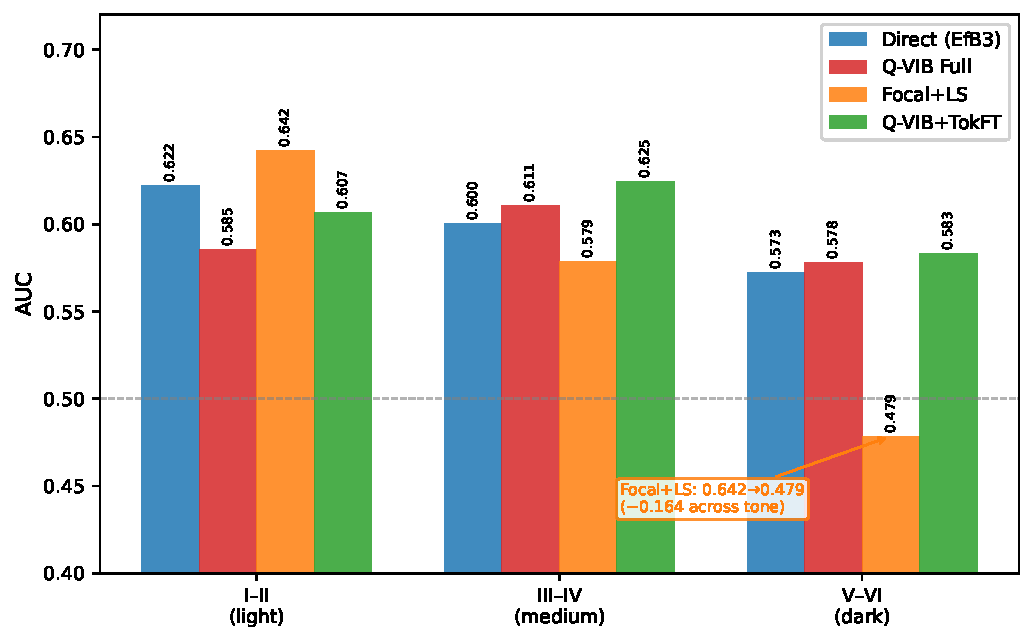
\includegraphics[width=0.7\linewidth]{../../report/figures/fig_fairness_fitz.pdf}
\caption{Per-skin-tone AUC on Fitzpatrick17k, stratified into light (I--II), medium (III--IV), and
dark (V--VI) tiers, for four methods. Source: \texttt{fairness\_fitzpatrick\_iclr\_full.csv}
(ICLR-exclusive re-run, R10-compliant; no BMVC fairness numbers are reused). All tiers show modest
absolute AUC because Fitzpatrick17k is a hard, diverse clinical pool; the salient signal is the
\emph{relative} gap across tones. The dark (V--VI) tier is lowest for every method, and Focal+LS falls
to $0.479$ on V--VI --- below the $0.5$ chance level --- with a light-to-dark drop of $-0.164$. We
report AUC differences only; no calibration metric is shown.}
\label{fig:fairness-fitz}
\end{figure}

\subsection{Cross-Source Generalisation}\label{app:crossdomain}

We next evaluate transfer across four distinct dermatology acquisition sources, reporting AUC per
source for the same four methods (Figure~\ref{fig:crossdomain}). Performance varies sharply with the
source: it is highest on HAM10000 ($0.805$ for the direct baseline), the source closest to the
training distribution, and degrades to near-chance on DermNet ($0.503$--$0.604$), the most distant and
heterogeneous source, with PAD-UFES and Fitzpatrick17k in between. This spread maps out both the
\emph{reach} of the system --- strong, near in-distribution transfer to HAM10000 --- and its
\emph{limits} --- transfer collapses towards chance on the hardest source. We deliberately do not
average these into a single headline figure, since doing so would obscure exactly the source-dependent
fragility that the analysis is meant to expose. As with the fairness analysis, the absolute values are
low because the pooled cross-source set is a genuinely difficult clinical mixture; we therefore read
the result as a map of where generalisation holds and where it does not, not as a claim of broad
robustness.

\begin{figure}[t]
\centering
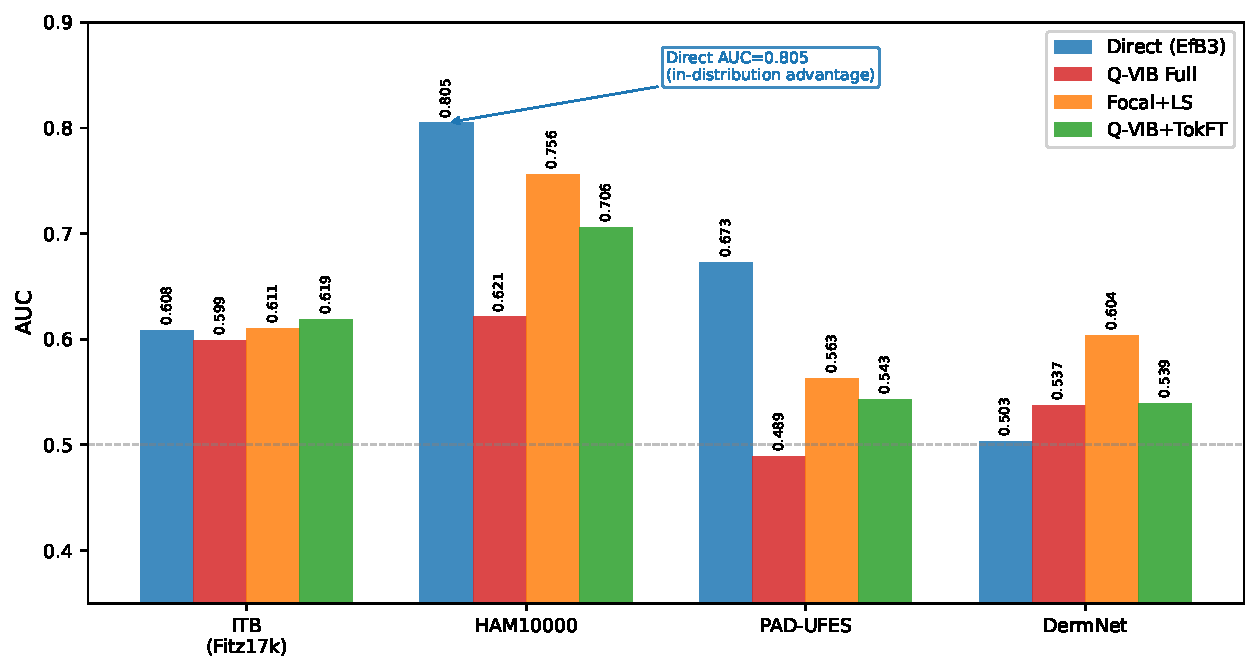
\includegraphics[width=0.7\linewidth]{../../report/figures/fig_crossdomain.pdf}
\caption{Cross-source AUC across four dermatology acquisition sources for four methods. Source:
\texttt{external\_*\_predictions.csv} (Jun14--15 ICLR re-run; per-source AUC independently recomputed,
R10-compliant; no BMVC cross-domain numbers are reused). Transfer is strongest on HAM10000 (closest to
the training distribution; $0.805$ for the direct baseline) and degrades to near-chance on DermNet
($0.503$--$0.604$, the most distant source), with PAD-UFES and Fitzpatrick17k intermediate. Absolute
AUC is low because the pooled cross-source set is a hard, diverse clinical mixture; the figure is read
as a map of the system's reach and its limits, not as a robustness claim. Values are not averaged into
a single headline, to avoid masking source-dependent fragility.}
\label{fig:crossdomain}
\end{figure}
